\documentclass[a4paper,11pt]{article}

% Kodovani (cestiny) v dokumentu: utf-8
%\usepackage[cp1250]{inputenc}	% Omezena stredoevropska kodova stranka, pouze MSW.
\usepackage[utf8]{inputenc}	% Doporucujeme pouzivat UTF-8 (unicode).

\usepackage[margin=2cm]{geometry}
\newtoks\jmenopraktika \newtoks\jmeno \newtoks\datum
\newtoks\obor \newtoks\skupina \newtoks\rocnik \newtoks\semestr
\newtoks\cisloulohy \newtoks\jmenoulohy
\newtoks\tlak \newtoks\teplota \newtoks\vlhkost

\jmenopraktika={Fyzikální praktikum 1}
\jmeno={Lukáš Lejdar}
\datum={12. března 2023}
\obor={F}
\skupina={Út 16:00}

\cisloulohy={7}
\jmenoulohy={Měření Poissonovy konstanty vzduchu}

\tlak={98.4970}
\teplota={21,1}
\vlhkost={47.4}

%%%%%%%%%%% Uzitecne balicky:
\usepackage[czech]{babel}
\addto\captionsczech{\renewcommand{\figurename}{Graf}}

\usepackage{graphicx}
\usepackage{amsmath}
\usepackage{xspace}
\usepackage{url}
\usepackage{indentfirst}
\usepackage{wrapfig}


%%%%%% Zamezeni parchantu:
\widowpenalty 10000 \clubpenalty 10000 \displaywidowpenalty 10000
%%%%%% Parametry pro moznost vsazeni vetsiho poctu obrazku na stranku
\setcounter{topnumber}{3}	  % max. pocet floatu nahore (specifikace t)
\setcounter{bottomnumber}{3}	  % max. pocet floatu dole (specifikace b)
\setcounter{totalnumber}{6}	  % max. pocet floatu na strance celkem
\renewcommand\topfraction{0.9}	  % max podil stranky pro floaty nahore
\renewcommand\bottomfraction{0.9} % max podil stranky pro floaty dole
\renewcommand\textfraction{0.1}	  % min podil stranky, ktery musi obsahovat text
\intextsep=8mm \textfloatsep=8mm  %\intextsep pro ulozeni [h] floatu a \textfloatsep pro [b] or [t]

% Tecky za cisly sekci:
\renewcommand{\thesection}{\arabic{section}.}
\renewcommand{\thesubsection}{\thesection\arabic{subsection}.}
% Jednopismenna mezera mezi cislem a nazvem kapitoly:
\makeatletter \def\@seccntformat#1{\csname the#1\endcsname\hspace{1ex}} \makeatother
%
\newcommand{\vsn}[4]{\ensuremath{#1 =} #2(#3)\,#4}
\newcommand{\vrn}[6]{\ensuremath{#1 =} (#2 $\pm$ #3)\,#4 ($p=$ #5\,\%, $\nu=$ #6)}

\renewcommand{\figurename}{Graf}

%%%%%%%%%%%%%%%%%%%%%%%%%%%%%%%%%%%%%%%%%%%%%%%%%%%%%%%%%%%%%%%%%%%%%%%%%%%%%%%
% Zacatek dokumentu
%%%%%%%%%%%%%%%%%%%%%%%%%%%%%%%%%%%%%%%%%%%%%%%%%%%%%%%%%%%%%%%%%%%%%%%%%%%%%%%

\begin{document}

\thispagestyle{empty}

{
\begin{center}
\sf 
{\Large Ústav fyziky a technologií plazmatu Přírodovědecké fakulty Masarykovy univerzity} \\
\bigskip
{\huge \bfseries FYZIKÁLNÍ PRAKTIKUM} \\
\bigskip
{\Large \the\jmenopraktika}
\end{center}

\bigskip

\sf
\noindent
\setlength{\arrayrulewidth}{1pt}
\begin{tabular*}{\textwidth}{@{\extracolsep{\fill}} l l}
\large {\bfseries Zpracoval:}  \the\jmeno & \large  {\bfseries Naměřeno:} \the\datum\\[2mm]
\large  {\bfseries Obor:} \the\obor  \hspace{40mm}  {\bfseries Skupina:} \the\skupina %
&\large {\bfseries Testováno:}\\
\\
\hline
\end{tabular*}
}

\bigskip

{
\sf
\noindent \begin{tabular}{p{4cm} p{0.6\textwidth}}
\Large  Úloha č. {\bfseries \the\cisloulohy:} \par
\smallskip
$T=\the\teplota$~$^\circ$C \par
$p=\the\tlak$~kPa \par
$\varphi=\the\vlhkost$~\%
&\Large \bfseries \the\jmenoulohy  \\[2mm]
\end{tabular}
}

\vskip1cm

\section{Úkoly}
\begin{enumerate}
  \item Pomocí U trubice ocejchujte diferenciální tlakové čidlo měřící proud 
\begin{align}
  p &=  p_0 + \rho g h \\
  I &= I_0 + c\Delta p
\end{align}
  \item Měření poissonovy konstanty Clément-Desormesovou metodou. Natlakujte velkou nádobu, změřte U-trubicí a průmyslovým tlakovým čidlem tlak před (p1) a po expanzi (p2) a spočítejte Poissonovu konstantu z obou čidel.
  \item Pro několik různých frekvencí určete vlnovou délku stojatého vlnění v Kundtově trubici. Pro každou frekvenci najděte všechny polohy maxim v trubici, vyneste je do grafu a stanovte vlnovou délku. Určete rychlost zvuku ve vzduchu a stanovte Poissonovu konstantu vzduchu včetně nejistoty měření.
\end{enumerate}

\subsection{Pomůcky}

\begin{itemize}
  \item Aparatura pro měření Clément Desormovou metodou
  \item Kundutova trubice
  \item frekvenční generátor
  \item svinovací metr
\end{itemize}
 
\section{Postup měření}

\subsection{Clément Desormova metoda}

Poissonova konstant vystupuje v adiabatckém ději jako,

\begin{equation}
  pV^{\kappa} = konst.
\end{equation}

Měření poissonovy konstanty přímo z tohoto vztahu by tedy vyžadovalo počkat na ustálení soustavy.
To je ale velmi těžko realizovatelné, když adiabatický děj probíhá v tepelné izolaci.

Clément-Desormova je způsob, jak se tomuto problému vyhout. 
Děj se bude nejprve skládat z adiabatické expanze ($p_1$, $T_1$) $\implies$ ($p_2$, $T_2$) .
Otevřeme ventil natlakované nádoby a po vyrovnání tlakú, ale minimální výměně tepla ho zase rychle uzavřeme. \\
\begin{equation}
  p_1^{\frac{1}{\kappa} -1} T_1 = p_2^{\frac{1}{\kappa} -1} T_2 \\
\end{equation}
Vzduch v nádobě je teď ochlazený adiabatickou expanzí a následuje izochorický ohřev okolím. \\ 


\begin{align}
  \frac{p_2}{T_2} &= \frac{p_3}{T_3}
\end{align}

,kde $T_3$ = $T_1$ je teplota okolí, $p_2$ tlak v laboratoři a $p_3$ tlak po ustanovení rovnováhy. 
Vyjádřením $\kappa$ a dosazením (1) pro tlak měřený U trubicí dostáváme,

\begin{equation}
  \kappa = \frac{\ln{\frac{p_1}{p_0}}}{\ln{\frac{p_1}{p_3}}} = \frac{\ln{\frac{p_0 + \rho g h_1}{p_0}}}{\ln{\frac{p_0 + \rho g h_1}{p_0 + \rho g h_3}}}.
\end{equation} \\

Taylorovým rozvojem,

\begin{equation}
  \kappa = \frac{h_1}{h_1 - h_3} + \frac{1}{2} \frac{h_1 h_3 \rho g}{p_0 (h_1 - h_3)} \ldots
\end{equation}

Je-li změna tlaku ve srovnání s atmosférickým tlakem dostatečně malá, pak

\begin{equation}
\kappa \approx \frac{h_1}{h_1 - h_3}
\end{equation}

Přesto že je tonto vztah aproximativní,
jeho výhodou je, že veličny, které zde vystupují pocházejǐ z jediného měřícího přístroje a absolutní chyby se můžou částečně pokrátit.

\subsection{Kundutova trubice}

Pro rychlost zvuku v ideálním plynu platí vztah

\begin{equation}
c = \sqrt{\kappa \frac{p}{\rho}} 
\end{equation}

, kde $p$ je tlak, $\rho$ hustota vzduchu a  $\kappa$ poissonova konstatnta. Ze stavové rovnice pro ideální plyn ale taky
\begin{equation}
  p = \frac{\rho R T}{ M_{mol}}
\end{equation}

Dosazení a vyjádřením $c$ dostáváme

 \begin{equation}
   \lambda f = \sqrt{\kappa \frac{RT}{M_{mol}}} 
\end{equation}

, kde $\lambda$ je vlnová délka a $f$ frekvence zvuku. 
Na generátoru sinusového signálu v Kundutově trubici nastavíme vhodnou frekvenci a zaznamenáváme polohy maximálních amplitud vlnění.
Rozdíl každých dvou maxim je polovina vlnové délky.

\newpage

\section{Výsledky měření}

\subsection{Kalibrace diferenciálního čidla}

\begin{table}[ht]
  \centering
  \begin{tabular}{ c | c }
     $I_0$ & $(4.09 \pm 0.05)$  [mA] \\ \hline
     c & $(0.031 \pm 0.001)$
  \end{tabular}
  \caption{Výsledky kalibrace z grafu \ref{fig:1}}
\end{table}

\subsection{Clément Desormovou metodou}

\begin{table}[ht]
  \centering
  \begin{tabular}{c | c }
    metoda & $\kappa$ \\ \hline\hline
    pomocí U trubice & $(1.31 \pm 0.04)$ \\
    pomocí kalibrace & $(1.32 \pm 0.04)$ \\ \hline
  \end{tabular}
  \caption{Hodnoty spočítané z grafu \ref{fig:2} a \ref{fig:3} Použitím vztahu (8)}
\end{table}

\subsection{Kundutovou trubicí}

Pro výpočet je potřeba tlak v laboratoři $p=98497.0$ Pa a hustota vzduchu, kterou zjistíme z online kalkulačky z odkazu [3]

\begin{table}[ht]
  \centering
  \begin{tabular}{c | c}
    $f$ [kHz] & $\kappa$ \\ \hline
    1.56 & $(1.4 \pm 0.2)$ \\
    1.89 & $(1.4 \pm 0.3 )$\\
    3.41 & $(1.40 \pm 0.03)$ \\
    5.04 & $(1.39 \pm 0.03)$ \\
  \end{tabular}
  \caption{Hodnoty spočítané z grafu \ref{fig:4}}
\end{table}

\section{Závěr}

Měření Clément Desormovou metodou nedopadlo nejlépe. Myslím, že jsem pokaždé zavřel ventil na nádobě moc brzo a tlaky se nestihli vyrovnat.
Proto je naměřená hodnota značně menší než skutečná. Měření Kundutovou trubicí je na druhou stranu docela přesné. 
Je i vidět, že pro větší hodnoty frekvence klesá vlnová délka což značně zjednodušuje hledání maxima a vede k přesnějšímu měření.



\begin{figure}[bp!]
  \centering
  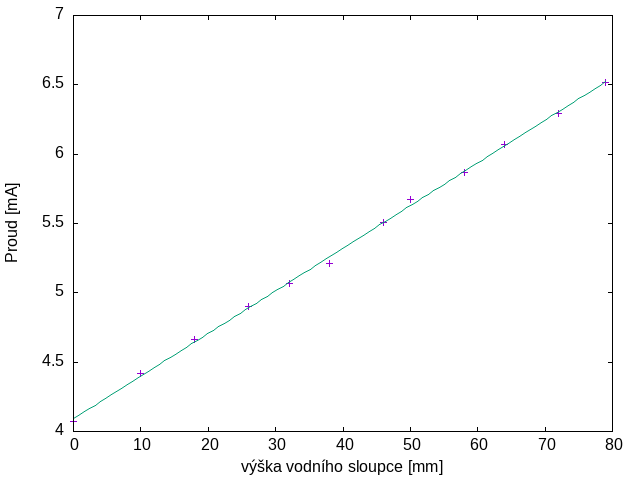
\includegraphics[width=0.7\linewidth]{kalibrace_proudu.png}
  \caption{závislost proudu protekájícího čidlem na výšce vodního sloupce od počáteční hodnoty}
  \label{fig:1}
\end{figure}

\begin{figure}[bp!]
  \centering
  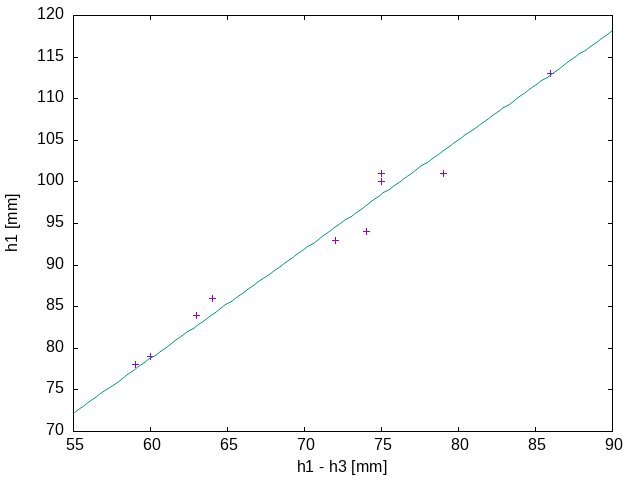
\includegraphics[width=0.7\linewidth]{clement.png}
  \caption{závislost rozdílu naměřených hodnot $h_1 - h_3$, na $h_1$}
  \label{fig:2}
\end{figure}


\begin{figure}[bp!]
  \centering
  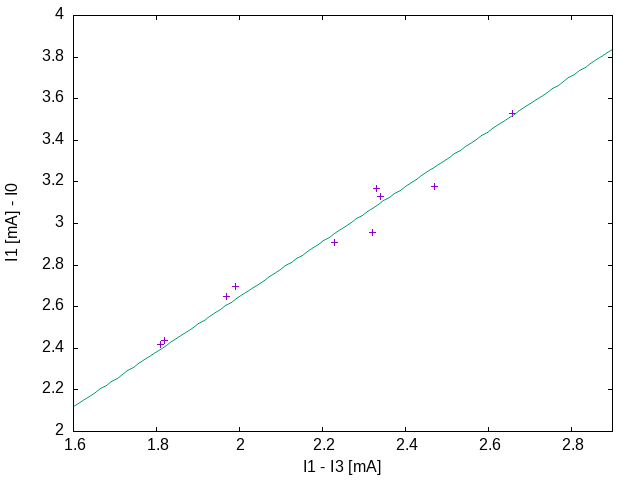
\includegraphics[width=0.7\linewidth]{clement-cidlem.png}
  \caption{závislost rozdílu naměřených hodnot $I_1 - I_3$, na $I_1 - I_0$}
  \label{fig:3}
\end{figure}

\begin{figure}[bp!]
  \centering
  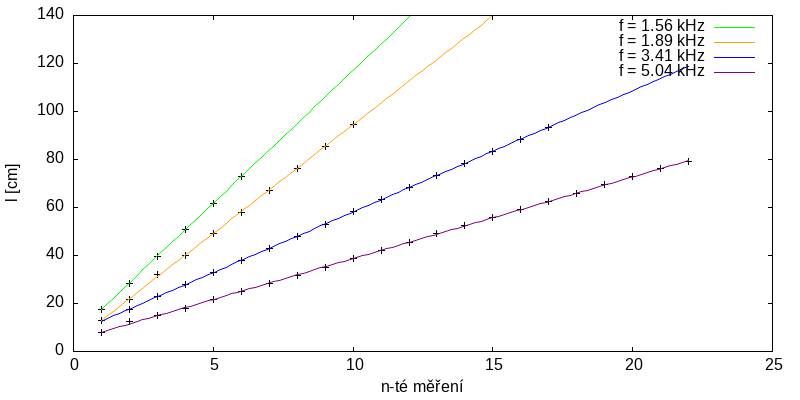
\includegraphics[width=0.9\linewidth]{vlnova_delka.png}
  \caption{závislost n-tého maxima amplitudy vlnění na vzdálenosti}
  \label{fig:4}
\end{figure}

\begin{thebibliography}{0}
\bibitem{navody} Bochníček a kol. \textit{Fyzikální praktikum 1, návody k ulohám.} Brno 2024.\\ Dostupné z~\url{https://monoceros.physics.muni.cz/kof/vyuka/fp1_skripta.pdf}.   
\bibitem{tabulky} Hustota pevných látek. Dostupné z~\url{http://www.converter.cz/tabulky/hustota-pevne.htmf}.   
\bibitem{hustota vzduchu} kalkulačka hustoty vzduchu \url{https://www.omnicalculator.com/physics/air-density}.
\end{thebibliography}

\end{document}

